% !TeX spellcheck = pl_PL
\documentclass[12pt]{oska}

% Lista wszystkich języków stanowiących języki pozycji bibliograficznych użytych w pracy.
% (Zgodnie z zasadami tworzenia bibliografii każda pozycja powinna zostać utworzona zgodnie z zasadami języka, w którym dana publikacja została napisana.)
\usepackage[english,polish]{babel}

% Użyj polskiego łamania wyrazów (zamiast domyślnego angielskiego).
\usepackage{polski}
\usepackage[utf8]{inputenc}

% dodatkowe pakiety
\usepackage{mathtools}
\usepackage{amsfonts}
\usepackage{amsmath}
\usepackage{amsthm}
\usepackage[dvipsnames]{xcolor}
\usepackage{textcomp}

% obrazki
\usepackage{graphicx}
\usepackage{rotating}
\usepackage{caption}
\usepackage{float}

% --- < bibliografia > ---

\usepackage[
style=numeric,
sorting=none,
% Zastosuj styl wpisu bibliograficznego właściwy językowi publikacji.
language=autobib,
autolang=other,
% Zapisuj datę dostępu do strony WWW w formacie RRRR-MM-DD
%urldate=iso,
%seconds=true,
% Nie dodawaj numerów stron, na których występuje cytowanie
backref=false,
% Podawaj ISBN.
isbn=true,
% Nie podawaj URL-i, o ile nie jest to konieczne
url=false,
% Ustawienia związane z polskimi normami dla bibliografii
maxbibnames=6,
minbibnames=6,
% Jeżeli używamy Bibera:
backend=biber
]{biblatex}

\AtBeginBibliography{
\renewcommand\labelnamepunct{:\space}
\renewcommand\newunitpunct{\addcomma\space}
\renewcommand{\finentrypunct}{}

\renewcommand{\bibopenparen}{\addcomma\addspace}
\renewcommand{\bibcloseparen}{\addspace}
}

\usepackage{csquotes}
% Ponieważ `csquotes` nie posiada polskiego stylu, można skorzystać z mocno zbliżonego stylu chorwackiego.
\DeclareQuoteAlias{croatian}{polish}

% Przecinki do numerów
\usepackage{icomma}
% ------------------------

% --- < listingi > ---

% Użyj czcionki kroju Times.
\usepackage{newtxtext}

\usepackage{listings}
\lstloadlanguages{TeX}

\lstset{
	literate={ą}{{\k{a}}}1
           {ć}{{\'c}}1
           {ę}{{\k{e}}}1
           {ó}{{\'o}}1
           {ń}{{\'n}}1
           {ł}{{\l{}}}1
           {ś}{{\'s}}1
           {ź}{{\'z}}1
           {ż}{{\.z}}1
           {Ą}{{\k{A}}}1
           {Ć}{{\'C}}1
           {Ę}{{\k{E}}}1
           {Ó}{{\'O}}1
           {Ń}{{\'N}}1
           {Ł}{{\L{}}}1
           {Ś}{{\'S}}1
           {Ź}{{\'Z}}1
           {Ż}{{\.Z}}1,
	basicstyle=\footnotesize\ttfamily,
}

% ------------------------

\AtBeginDocument{
	\renewcommand{\tablename}{\textbf{Tabela}}
	\renewcommand{\figurename}{\textbf{Rysunek}}
}

% ------------------------
% --- < tabele > ---

\usepackage{array}
\usepackage{tabularx}
\usepackage{multirow}
\usepackage{booktabs}
\usepackage{makecell}
\usepackage[flushleft]{threeparttable}

% defines the X column to use m (\parbox[c]) instead of p (`parbox[t]`)
\newcolumntype{C}[1]{>{\hsize=#1\hsize\centering\arraybackslash}X}

\setlength{\cftsecnumwidth}{10mm}
\setcounter{secnumdepth}{4}
\brokenpenalty=10000\relax

%---------------------------------------------------------------------------

%---------------------------------------------------------------------------

\titlePL{Wybrane aspekty modyfikacji obudowy zestawu głośnikowego}
\titleEN{Selected Aspects of Loudspeaker Cabinet Modifications}
\affiliation{Akademia Górniczo-Hutnicza im. S. Staszica w Krakowie}

%------------------------------------AUTORZY-----------------------

\namem{Michał}
\surnamem{Kmiecik}
\email{miszkoo@gmail.com} % adres do korespondencji -- zazwyczaj głównego autora

% Jeśli jesteś jedynym autorem pracy - pozostaw poniższe pola puste

\namei{Teresa}
\surnamei{Makuch}

\nameii{}
\surnameii{}
\nameiii{}
\surnameiii{}
\nameiiii{}
\surnameiiii{}
\nameiiiii{}
\surnameiiiii{}

%--------------------------STRESZCZENIE------------------------

\summaryPL{W procesie projektowania zestawu głośnikowego równie duże znaczenie, jak dobór przetworników, mają własności obudowy. Celem pracy było zbadanie wpływu różnych modyfikacji obudowy zestawu głośnikowego na jego parametry. W~związku z~tym wykonano pomiary impedancji elektrycznej, charakterystyk kierunkowości i~skuteczności zestawu, z~zastosowaniem różnych modyfikacji obudowy. Zarejestrowano także przebiegi drgań obudowy przy pomocy wibrometru laserowego. W~celu prowadzenia dalszych badań drogą symulacji, wykonano model komputerowy badanego zestawu przy użyciu metody elementów skończonych (MES). Podczas pomiarów zauważono znaczącą rozbieżność wyników z~danymi udostępnionymi przez producenta. W~związku z~tym przeprowadzono pomiary mające na celu weryfikację parametrów podanych w~karcie katalogowej. W~pracy zaprezentowano uzyskane wyniki, a~także spostrzeżenia związane z~wielokrotnym pomiarem i~zmiennością parametrów nowego przetwornika na skutek eksploatacji.}

\summaryEN{When designing a~loudspeaker, both the choice of transducers used and the cabinet characteristics are important. The authors’ aim was to investigate how different cabinet modifications influence the loudspeaker’s parameters. Therefore, loudspeakers' electric impedance, directivity characteristics and sensitivity were measured, covering various cabinet modifications. Vibrations of the cabinet were also recorded, using a laser vibrometer. In order to continue the research by simulation, a~computer model of the cabinet under inquiry was created using the finished elements method (FEM). During measurements, inconsistency between the obtained results and the producer’s data was discovered. Therefore, measurement aiming to verify parameters contained in data sheet was performed. The study presents obtained results and remarks on multiple measurement and fluctuation of a~new transducer’s parameters due to exploitation.}

%---------------------------------------------------------
% Nazwa pliku z bibliografią
%---------------------------------------------------------
\addbibresource{refs_OSKA.bib}
%---------------------------------------------------------
%pauza przy podawaniu zakresu liczb
\newcommand{\range}[2]{\num{#1}~--~\num{#2}}
%komentarze
\newcommand{\comment}[1]{{\color{magenta}\emph{\textbf{#1}}}}
%---------------------------------------------------------
%obrazki
%---------------------------------------------------------
\usepackage{adjustbox}
\graphicspath{{./}{obrazki/}}


\begin{document}

\maketitles

\section{Wstęp}

	\comment{Co w ogóle robimy, po co (może coś w~stylu, że chcieliśmy bardziej projektować, a~wyszło, że bardziej mierzyliśmy), plus trochę teorii (w~zależności, ile miejsca zajmie nam reszta...)}
	
	\subsection{Wprowadzenie teoretyczne}
	
	\comment{O zależnościach (?) z inżynierki}
	
	\subsection{Cel pracy}
	
		Autorzy postawili sobie za cel określenie, jakie z~zastosowanych modyfikacji obudowy zestawu głośnikowego wywierają wpływ na jego mierzone parametry oraz wybór najbardziej optymalnej konfiguracji, a~także wyznaczenie optymalnego punktu podziału pasma częstotliwości między głośniki. \comment{Zweryfikować, czy jest spełniony! Ew. włączyć do wstępu jako 1 części, bez podziału na podsekcje.}

\section{Badany zestaw głośnikowy}

	\subsection{Opis konstrukcji}\label{ss:opis}
	
		Zestaw, którego parametry zdecydowano się zbadać, i~który poddano modyfikacjom, jest docelowo elementem systemu liniowego. Składa się z~falowodu z~wysokotonowym głośnikiem ciśnieniowym B\&C~DE800 umieszczonego centralnie oraz dwóch głośników nisko-średniotonowych Beyma~10WR300 umieszczonych po bokach i~nachylonych pod kątem \SI{67}{\degree} do osi głównej zastawu. 
		
		Obudowa ma kształt typowy dla systemu liniowego -- przekrój boczny jest w~kształcie trapezu równoramiennego; konstrukcja wzorowana jest na rozwiązaniu stosowanym w~systemie liniowym uznanej firmy. Materiał korpusu to sklejka bałtycka o~grubości \SI{15}{\milli\metre}, dodatkowo z~przodu zamontowana jest maskownica ze stali o~grubości \SI{2}{\milli\metre}. Objętość wnętrza obudowy po odjęciu objętości głośników i~falowodu wynosi \SI{28,17}{\litre}.
		
		Obudowa jest obudową wentylowaną, wyposażoną w~4~otwory o~kształcie ćwierćkolistym i~promieniu \SI{70}{\milli\metre}. Otwory te mają swe ujście do przestrzeni przed głośnikiem, tak jak przestawiono na rysunku~\ref{r:przekroj}. %Wnętrze obudowy jest połączone z~przestrzenią zewnętrzną półkolistymi otworami o~promieniu \SI{70}{\milli\metre} przy tylnej ściance.
		Taki układ głośników i~otworów ma wpływ na charakterystyki kierunkowości głośnika w~płaszczyźnie horyzontalnej~\cite{kmiecik_inz}. \comment{W części teoretycznej wzorek na chke kierunkowości w zależności od odległości źródeł i omówić temat!!!}
		
	%	Przekrój zestawu w~płaszczyźnie poziomej ukazano na rysunku~\ref{r:przekroj}, a~fotografię na rysunku~\ref{r:zdjecie}.
		
		\begin{figure}[!ht]
			\centering
			\adjincludegraphics[width=\textwidth,trim={{.1\width} {.25\height} {.17\width} {.12\height}},clip]{render_z_otworami_bez_tekstury.pdf}
			\caption{Przekrój modelu badanego zestawu głośnikowego w~płaszczyźnie poziomej wykonany w~programie Inventor}
			\label{r:przekroj}
		\end{figure}
		
		\begin{figure}[!ht]
			\centering
% 			\includegraphics[width=.8\textwidth]{}
			\caption{Fotografia badanego zestawu głośnikowego}
			\label{r:zdjecie}
		\end{figure}
	
	\subsection{Modyfikacje obudowy}
	
		W~celu określenia wpływu konstrukcji obudowy na parametry zestawu głośnikowego zastosowano wybrane rodzaje jej modyfikacji. Wybrano modyfikacje możliwe do faktycznego zastosowania, a~jednocześnie takie, które nie wymagają nieodwracalnej ingerencji w~obudowę.
		
		Oprócz modyfikacji obudowy, zmieniano także liczbę zamontowanych w~niej głośników, aby lepiej zbadać ich wzajemny wpływ. Wszystkie konfiguracje pomiarowe opisano w~tabeli~\ref{t:obudowa}.
		
		\begin{table}[!ht]
			\centering
			\caption{Opis konfiguracji obudowy i~głośników wykorzystanych podczas pomiarów}
			\label{t:obudowa}
			\begin{tabular}{|c|c|m{.6\textwidth}|}
				\hline
				\textbf{L.p.} & \makecell{\textbf{Oznaczenie}\\\textbf{(na wykresach)}} & \centering\textbf{Opis} \tabularnewline\hline
				1. & Pusta & Obudowa w~podstawowej wersji (opisanej w~części~\ref{ss:opis}), z~otworami, bez wypełnienia \\\hline
				2. & Wypełniona & Wnętrze obudowy wypełnione materiałem dźwiękochłonnym z~włókien poliestrowych umieszczonym na ściankach \\\hline
				3. & Zaślepiona & Ćwierćkoliste otwory zaślepione elementami ze sklejki o~grubości \SI{6,4}{\milli\metre}, przyklejonymi do ścianki, w~której zamocowany jest głośnik niskotonowy\\\hline
				\hline
				4. & Jeden głośnik & Jeden głośnik niskotonowy zamocowany w~obudowie, otwór na drugi zaślepiony kołem ze sklejki; zamocowany głośnik wysokotonowy \\\hline
				5. & Dwa głośniki & Obydwa głośniki niskotonowe oraz głośnik wysokotonowy zamocowane w~obudowie\\\hline
			\end{tabular}
		\end{table}

\section{Metodyka pomiarów}

	W~celu możliwie dokładnego zbadania parametrów zestawu, ze szczególnym uwzględnieniem obudowy, zaplanowano szereg pomiarów: impedancji elektrycznej głośnika w~odgrodzie z~wyznaczeniem parametrów Thiele-Smalla, charakterystyki skuteczności, charakterystyk kierunkowości oraz pomiar drgań obudowy przy pomocy wibrometru laserowego -- metodykę wymienionych pomiarów opisano w~części~\ref{ss:metodyka}.
	
	Ze względu na zaobserwowane znaczące rozbieżności między wynikami uzyskanymi dla głośników niskotonowych, a~parametrami podanymi przez producenta w~karcie katalogowej, zdecydowano się na wykonanie dodatkowych pomiarów, uwzględniających zużycie głośnika; pomiary te opisano w~części~\ref{ss:dodatkowe}.
	
	Metodyka pomiarów opierała się na wytycznych zawartych w~normie EN~60268-5~\cite{norma}. Natężenie prądu elektrycznego i~napięcie elektryczne tam, gdzie to było konieczne, monitorowano przy pomocy multimetrów Tektronix DMM~4040 oraz DMM~4050.

	\subsection{Metodyka podstawowa}\label{ss:metodyka}
	
		\subsubsection{Impedancja elektryczna i parametry Thiele-Smalla}
			
			Pomiary wykonano przy pomocy systemu Brüel\&Kjær Pulse, pozwalającego na pomiar charakterystyki impedancji oraz wyznaczenie na tej podstawie parametrów Thiele-Smalla.
			
			Do wyznaczenia tych parametrów wykorzystano metodę dodanej masy: wykonano pomiar impedancji głośnika, a~następnie do membrany dodano masę $m=\,$\SI{10}{\gram} i~wykonano kolejny pomiar. Na podstawie porównania dwóch charakterystyk impedancji, za pomocą dedykowanego oprogramowania Pulse Thiele Small Parameters Calculation BZ-5604 wyznaczano parametry Thiele-Smalla~\cite{BK_pulse_TS}, opisane w~tabeli~\ref{t:TS_opis}.
			
			Istnieją dwie metody pomiaru parametrów Thiele-Smalla: metoda dodanej masy oraz metoda dodanej objętości. Ze względów praktycznych zdecydowano się na wykonywanie większości pomiarów metodą dodanej masy, dla porównania wykonano też jeden pomiar metodą dodanej objętości.
			
			\begin{table}[!ht]
				\centering
				\caption{Parametry Thiele-Smalla}
				\label{t:TS_opis}
				\begin{tabular}{|c|c|c|}
				\hline
					\textbf{Oznaczenie} & \textbf{Jednostka} & \textbf{Opis parametru}\\\hline\hline
					\multicolumn{3}{|c|}{Parametry wyznaczane z pojedynczego pomiaru} \\\hline\hline
					$F_s$ & \si{\hertz} & Częstotliwość rezonansowa \\\hline
					$Z_{max}$ & \si{\ohm} & Impedancja w~rezonansie \\\hline
					$R_e$ & \si{\ohm} & Rezystancja dla napięcia stałego \\\hline
					\gape{$r_0=\frac{Z_{max}}{R_e}$} & --- & Stosunek impedancji cewki do rezystancji \\\hline
					$S$ & \% & \makecell{Symetria rezonansu, wyznacznik wiarygodności\\obliczonych parametrów -- powinna wynosić najwyżej 3,5\%} \\\hline
					\hline
					$Q_{ms}$ & --- & Dobroć mechaniczna \\\hline
					$Q_{es}$ & --- & Dobroć elektryczna \\\hline
					\gape{$Q_{ts}=\frac{Q_{ms}\cdot Q_{es}}{Q_{ms}+Q_{es}}$} & --- & Dobroć całkowita \\\hline
					\hline
					\multicolumn{3}{|c|}{Parametry wyznaczane z dwóch pomiarów (samej membrany i z dodaną masą)} \\\hline\hline
					$V_{as}$ & \si{\litre} & Równoważna objętość podatności głośnika \\\hline
					$M_{ms}$ & \si{\gram} & Masa mechaniczna membrany \\\hline
					$C_{ms}$ & \si[per-mode=symbol]{\metre\per\newton} & Podatność mechaniczna zawieszenia \\\hline
					$R_{ms}$ & \si[per-mode=symbol]{\metre\per\newton} & Rezystancja mechaniczna głośnika \\\hline
					\hline
					$M_{as}$ & \si[per-mode=symbol]{\kilo\gram\per\metre\tothe{4}} & Masa akustyczna membrany \\\hline
					$C_{as}$ & \si[per-mode=symbol]{\metre\tothe{5}\per\newton} & Podatność akustyczna zawieszenia \\\hline
					$R_{as}$ & \si[per-mode=symbol]{\newton\s\per\metre\tothe{5}} & Rezystancja akustyczna głośnika \\\hline
					\hline
					$\eta_0$ & \% & Sprawność głośnika \\\hline
					$Bl$ & \si{\tesla\metre} & \makecell{Współczynnik przetwarzania elektromechanicznego\\(indeks siły)} \\\hline
					$L_{e} (1\si{\kilo\hertz})$ & \si{\henry} & Indukcyjność cewki dla częstotliwości \SI{1}{\kilo\hertz} \\\hline
				\end{tabular}
			\end{table}

			
			Pomiar wykonano z~użyciem sygnału sinusoidalnego z~krokiem $1/24$~oktawy w~zakresie \range{}{}~\si{\hertz}.
			
% 			Zmierzono impedancję głośnika niskotonowego w~odgrodzie, jednego głośnika w~obudowie oraz obu głośników w~obudowie.
			Zmierzono impedancję głośnika niskotonowego w~odgrodzie oraz głośników w~obudowie z~zastosowanymi różnymi modyfikacjami. 
			
			
			
		\subsubsection{Charakterystyka skuteczności}
			
			Do pomiarów wykorzystano analizator SVAN~912~E; głośnik pobudzano szumem różowym z~generatora o~wartości skutecznej \SI{1}{\watt}. Analizę prowadzono w~odległości \SI{2}{\metre} w~pasmach $1/3$-oktawowych w~zakresie \range{50}{5000}~\si{\hertz}.
			
		\subsubsection{Skuteczność}
		
			\comment{ewentualnie w całość char + jednoliczbowa}
			
		\subsubsection{Charakterystyki kierunkowości}
			
			Wykonano dwie serie pomiarów, dla głośnika wysoko- i~niskotonowego. W~pierwszej serii zmierzono głośniki w~obudowie bez wypełnienia, w~drugiej -- wypełnione materiałem dźwiękochłonnym.
			
			Pomiar charakterystyki kierunkowości odbywał się w~komorze bezechowej przy użyciu stolika obrotowego, na którym umieszczony był zestaw głośnikowy. W~osi akustycznej mierzonego głośnika ustawiono mikrofon GRAS 46AE; następnie głośnik obracano z~krokiem \SI{10}{\degree}, każdorazowo zatrzymując i~wykonując pomiar trwający \SI{3}{\s}. Sygnałem podawanym na głośnik był szum różowy, pomiar wykonano w~pasmach $1/6$~oktawy, w~zakresie \range{40}{20000}~\si{\hertz}.
			
		\subsubsection{Drgania obudowy}
			
			Pomiar drgań obudowy miał na celu sprawdzenie, w~jakim stopniu charakterystyka częstotliwościowa zestawu jest związana z~właściwościami obudowy. Badany zestaw głośnikowy umieszczono w~komorze bezechowej; w~wybranych punktach (por.~\ref{r:wibro_pkt}) naklejono taśmę odblaskową, na którą padała wiązka lasera; zastosowanie taśmy było niezbędne dla uzyskania odpowiedniego odbicia światła od badanych powierzchni. %Wibrometr umieszczono w~odpowiedniej odległości, tak aby uniknąć przesterowania sygnału. 
			Sygnałem pomiarowym był szum różowy, rejestrowano jednocześnie przebieg drgań wibrometrem oraz sygnał akustyczny dwoma mikrofonami: jednym umieszczonym blisko bieżącego punktu pomiarowego (rys.~\ref{r:wibro_zdjecie}), a~drugim w~odległości~\SI{2}{\metre}. Wibrometr umieszczono poza przestrzenią komory celem zapewnienia jego stabilnego usadowienia.
			
			\begin{figure}[!ht]
				\centering
				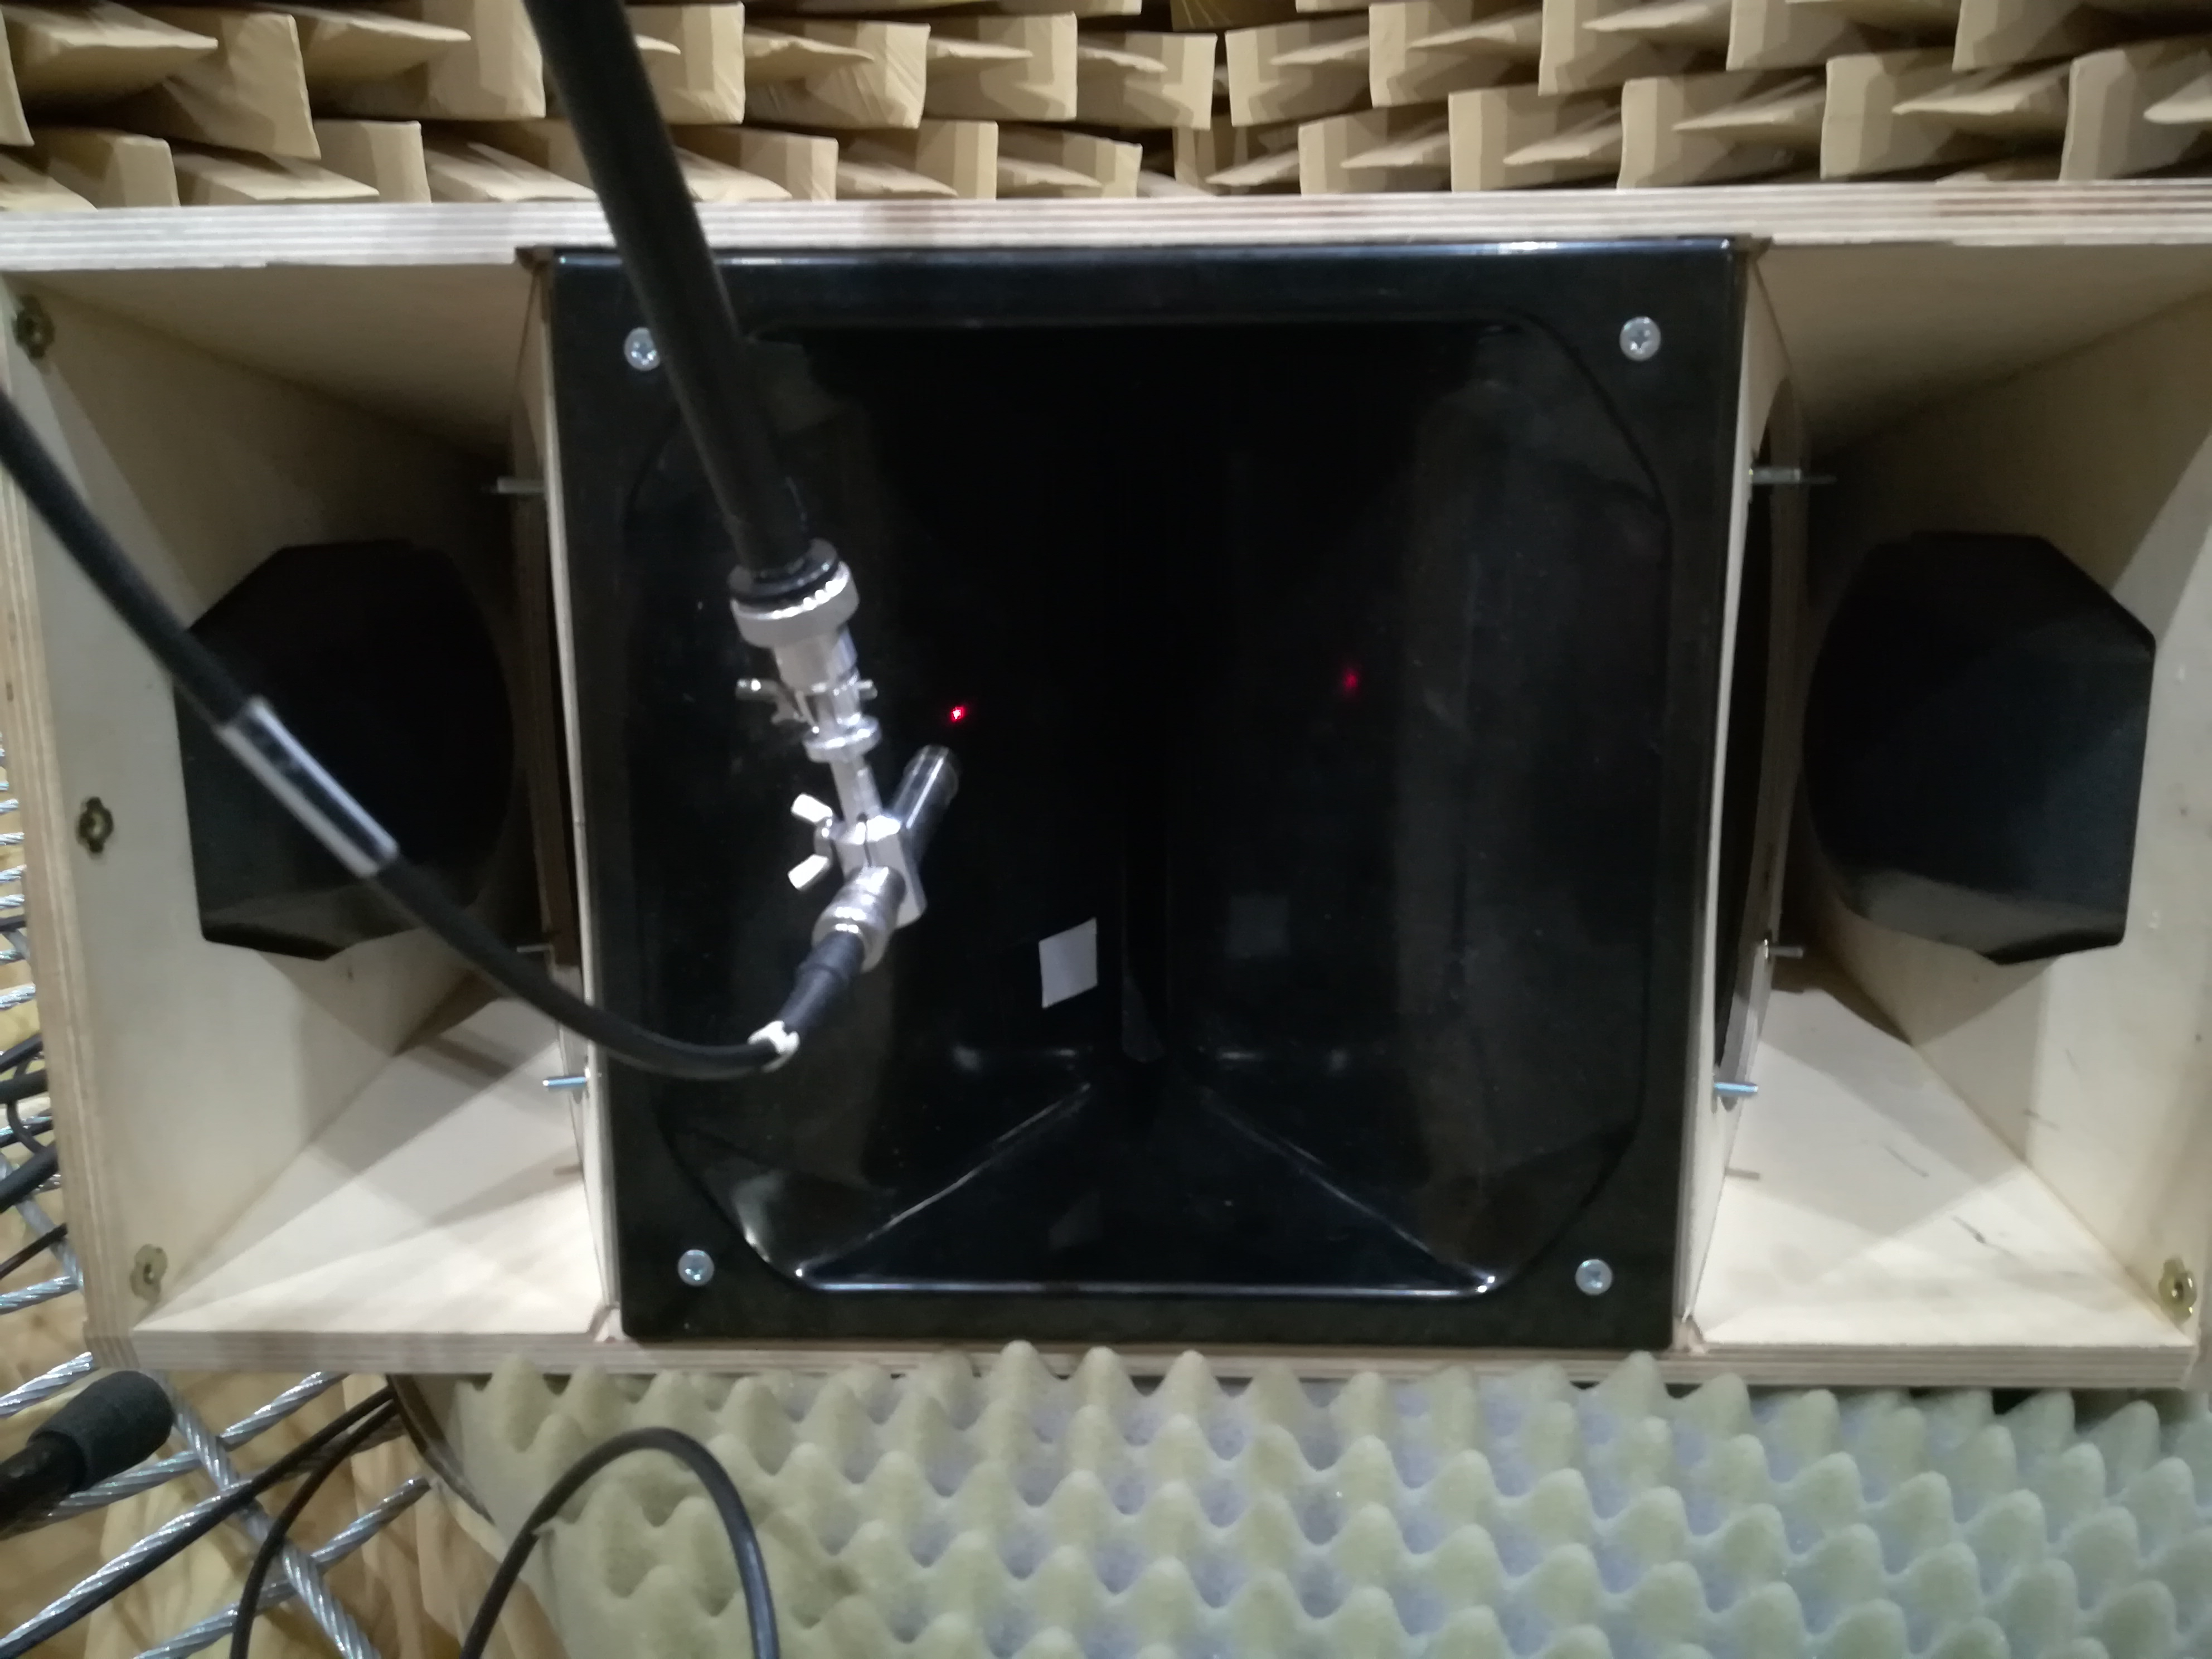
\includegraphics[width=.8\textwidth]{zdjecie_wibro.jpg}
				\caption{Fotografia wykonana podczas przygotowań do pomiaru z~użyciem wibrometru}
				\label{r:wibro_zdjecie}
			\end{figure}

	
% 	\subsection{Dodatkowe pomiary}\label{ss:dodatkowe}

\section{Modelowanie}

	\comment{Opis modelu w Comsolu, co modelowaliśmy, metody (?). To pisze Michał...}

\section{Analiza wyników}

	\subsection{Pomiary impedancji}
		
		Na rysunku \ref{r:metody} przedstawione zostały przebiegi impedancji w~funkcji częstotliwości uzyskane dla obu metod. 
		
		\begin{figure}[!ht]
			\centering
			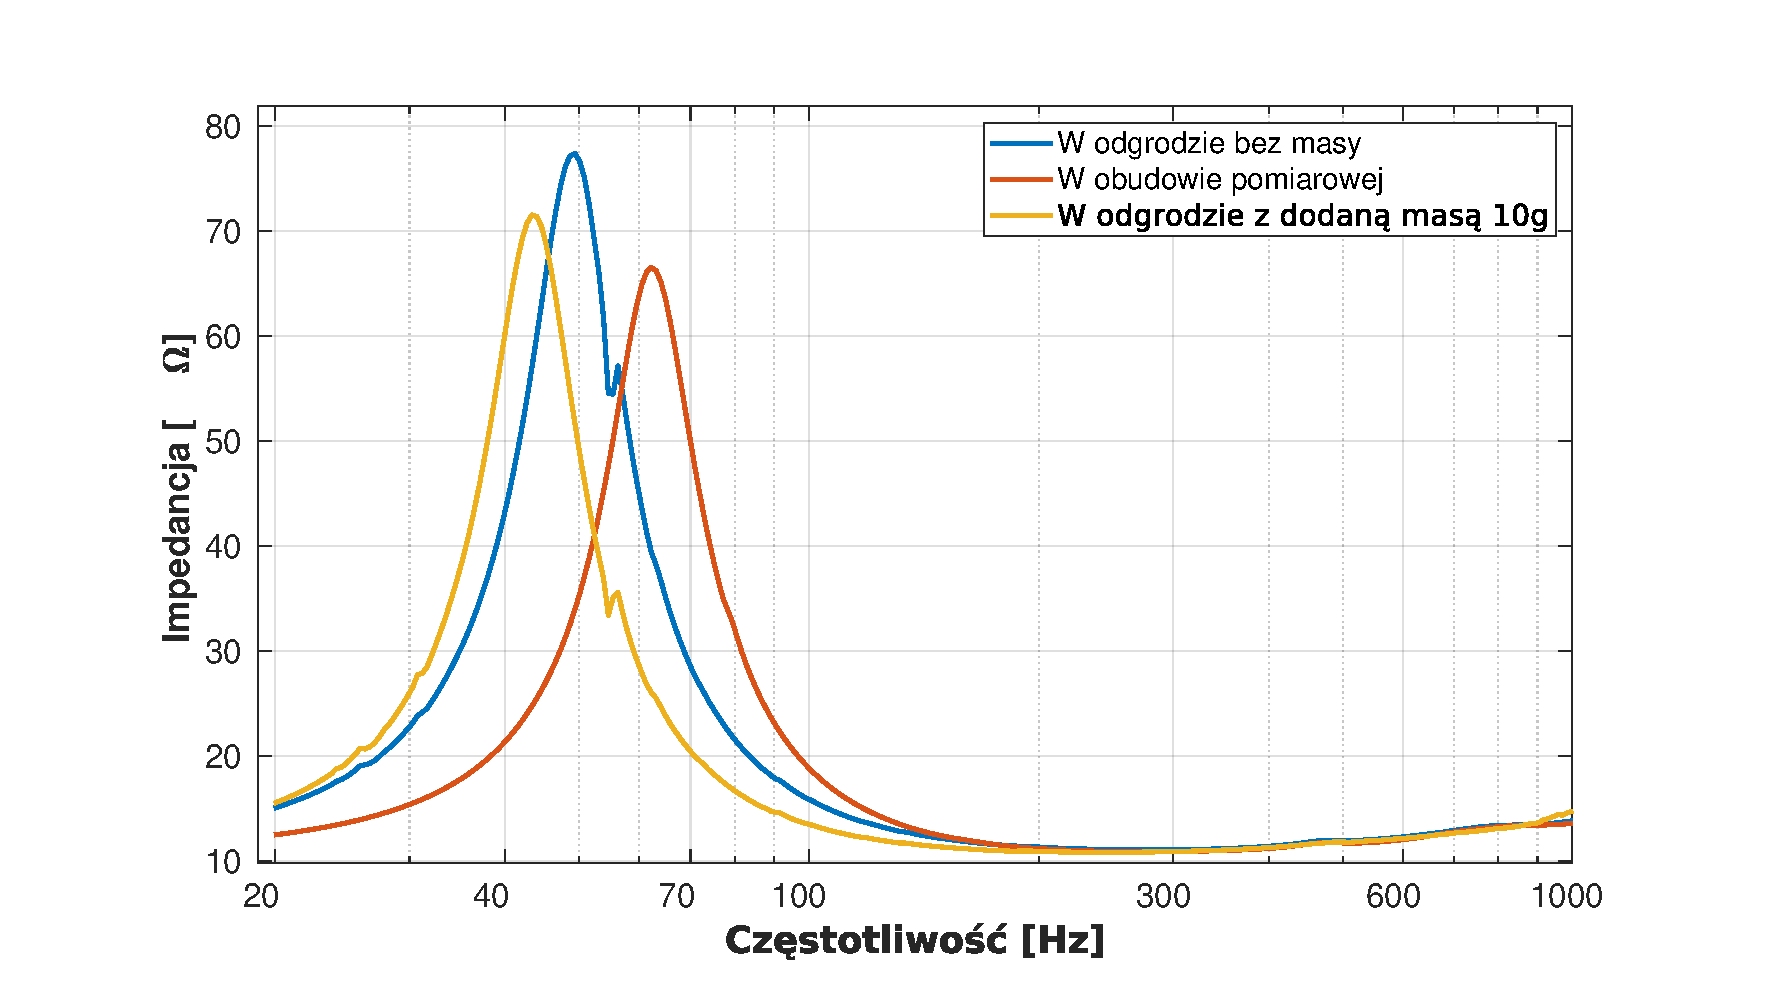
\includegraphics[width=.8\textwidth,trim={2cm .5cm 2cm 1cm},clip]{metody_2glosnik.pdf}
			\caption{\comment{Czy ten rysunek nam jest potrzebny???}}
			\label{r:metody}
		\end{figure}
		
		\begin{figure}[!ht]
			\centering
			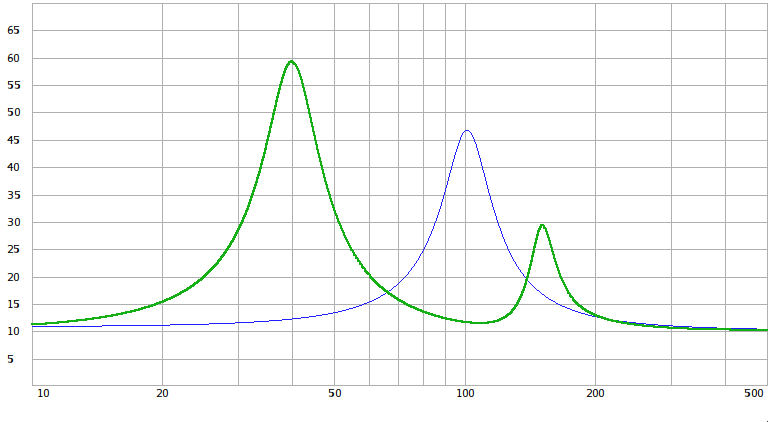
\includegraphics[width=.9\textwidth]{obrazki/winisd_screen.png}\\
			\setlength{\unitlength}{1mm}
			\begin{picture}(0,0)
				\put(-6,4){\texttt{$f$ [Hz]}}
				\put(-78,40){\rotatebox{90}{$Z_e [\Omega]$}}
			\end{picture}
			\caption{Wyniki symulacji impedancji dwóch głośników w~obudowie w~programie WinISD; \color{Green}zielony\color{Black} -- obudowa z~otworami; \color{Blue}niebieski\color{Black} -- zaślepione otwory}
			\label{r:winisd}
		\end{figure}
		
		\begin{figure}[!ht]
			\centering
			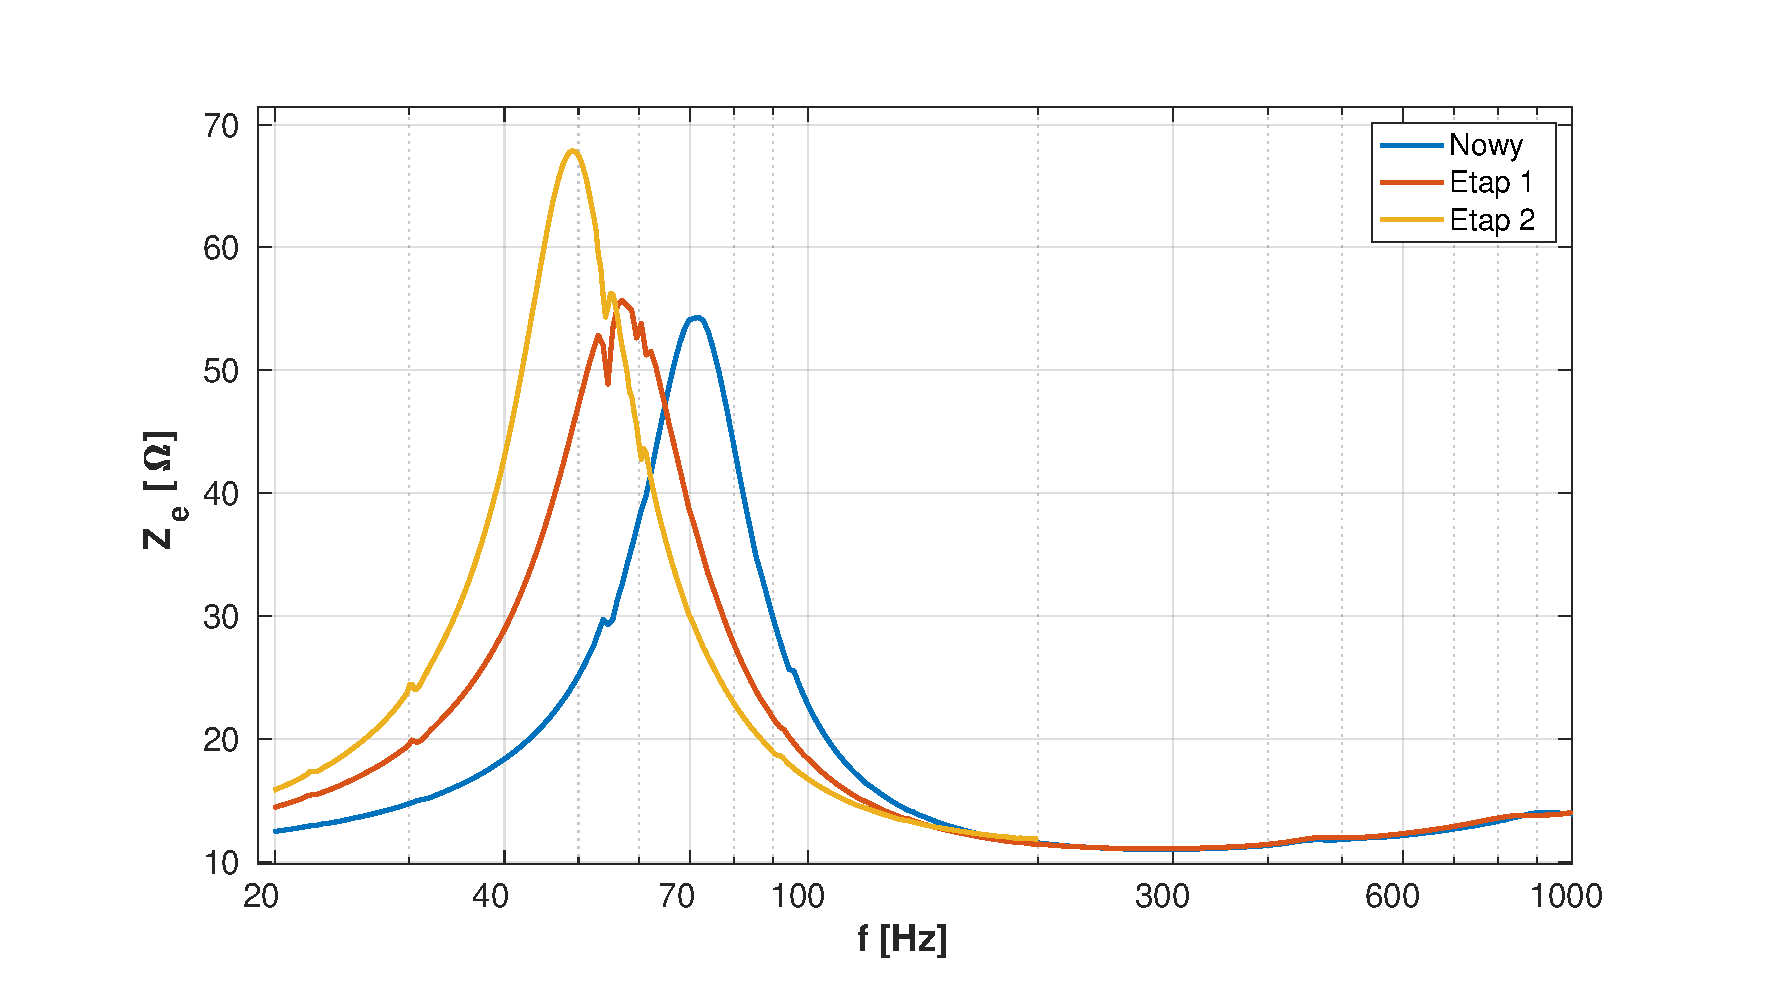
\includegraphics[width=.8\textwidth,trim={2cm .5cm 2cm 1cm},clip]{odgroda_wygrzewanie.pdf}
			\caption{}
			\label{r:wygrzewanie}
		\end{figure}
		
		Z~przyczyn technicznych parametry T-S dla tego pomiaru zostały obliczone na podstawie dostępnych materiałów (\cite{dobrucki},), a~nie wyznaczone przy pomocy systemu Pulse.
		
		\begin{table}[!ht]
			\centering
			\caption{Porównanie parametrów Thiele-Smalla: odczytanych z~karty katalogowej oraz zmierzonych metodą dodanej masy ($m=$~\SI{10}{\gram}) dla różnych etapów pracy głośnika}
			\label{t:TS_karta_etapy}
			\boldmath
			\begin{tabular}{|c|c|c|c|c|}
				\hline
				\textbf{Parametr} & \makecell{\textbf{Karta katalogowa}\\ \textbf{($R=$~\SI{8}{\ohm})}} & \textbf{Fabryczny} & \textbf{Etap 1} & \textbf{Etap 2} \\\hline
				\hline
				$F_s$ [\si{\hertz}] & \num{47,0}  & \num{71,5} & \num{57,0} & \num{50,7}  \\\hline
				$Z_{max}$ [\si{\ohm}] & --- & \num{54,2} & \num{55,7} & \num{64,0}  \\\hline
				$R_e$ [\si{\ohm}] & \num{6,1}  & \num{10,4} & \num{10,0} & \num{10,2}  \\\hline
				$r_0$ & ---  & \num{5,2} & \num{5,6} & \num{6,4} \\\hline
				$S$ [\%] & ---  & \num{3,44}  & \num{3,35} & \num{0,55} \\\hline
				\hline
				$Q_{ms}$ & \num{3,9}  & \num{3,3} & \num{2,7} & \num{2,8} \\\hline
				$Q_{es}$ & \num{0,4}  & \num{0,8} & \num{0,6} & \num{0,5} \\\hline
				$Q_{ts}$ & \num{0,3}  & \num{0,6} & \num{0,5} & \num{0,4} \\\hline
				\hline
				$V_{as}$ [\si{\litre}] 								& \num{50,9}  & \num{23,5} & \num{34,5} & \num{41,4} \\\hline
				$M_{ms}$ [\si{\gram}] 								& \num{39,0}  & \num{36,1}  & \num{38,5} & \num{40,6} \\\hline
				$C_{ms}$ [\si[per-mode=symbol]{\metre\per\newton}] 	& \num{294e-6}  & \num{138e-6}  & \num{203e-6} & \num{243e-6} \\\hline
				$R_{ms}$ [\si[per-mode=symbol]{\metre\per\newton}] 	& \num{2,9}  & \num{5,0}  & \num{5,2} & \num{4,6} \\\hline
				\hline
				$M_{as}$ [\si[per-mode=symbol]{\kilo\gram\per\metre\tothe{4}}] 	& \num{31,8}  & \num{30,1}  & \num{32,1} & \num{33,8} \\\hline
				$C_{as}$ [\si[per-mode=symbol]{\metre\tothe{5}\per\newton}] 	& \num{0,4e-6}  & \num{0,2e-6} & \num{0,2e-6} & \num{0,3e-6}  \\\hline
% 				$C_{as}$ [\si[per-mode=symbol]{\metre\tothe{5}\per\newton}] & \num{360e-9} & \num{165e-9} & \num{243e-9} & \num{292e-9} \\\hline
				$R_{as}$ [\si[per-mode=symbol]{\newton\s\per\metre\tothe{5}}] 	& \num{2367}  & \num{4123}  & \num{4323} & \num{3790} \\\hline
				\hline
				$\eta_0$ [\%] & \num{1,5}  & \num{1,08} & \num{1,07} & \num{1,00}   \\\hline
				$Bl$ [\si{\tesla\metre}] & \num{14,2} & \num{14,7} & \num{15,4} & \num{15,7}\\\hline
				$L_{e} (1\si{\kilo\hertz})$ [\si{\henry}] & \num{1e-3} & \num{1,984e-3} & \num{880e-6} & \num{911e-6} \\\hline
			\end{tabular}
			\unboldmath
		\end{table}
		
		\begin{table}[!ht]
			\centering
			\caption{Porównanie metod pomiaru parametrów Thiele-Smalla: dodanej masy oraz objętości}
			\label{t:TS_metody}
			\boldmath
			\begin{tabular}{|c|c|c||c|c|}
				\hline
				\multirow{2}{*}{\textbf{Parametr}} & \multicolumn{2}{c|}{\textbf{Etap 1, głośnik 1}} & \multicolumn{2}{|c|}{\textbf{Etap 2, głośnik 2}}\\\cline{2-5}
				& \textbf{Masa \SI{5}{\gram}} & \multicolumn{2}{c|}{\textbf{Masa \SI{10}{\gram}}} & \textbf{Obudowa \SI{80}{\litre}}\\\hline
				\hline
				$F_s$ [\si{\hertz}] 	& \num{56,5} & \num{57,0} & \num{49,2} & \num{50,1} \\\hline
				$Z_{max}$ [\si{\ohm}] 	& \num{57,2} & \num{55,7} & \num{77,5} & \num{73,7} \\\hline
				$R_e$ [\si{\ohm}] 		& \num{10,0}  & \num{10,0} & \num{10,1} & \num{10,1} \\\hline
				$r_0$ 					& \num{5,7} & \num{5,6} & \num{7,8} & \num{7,4}\\\hline
				$S$ [\%]				& \num{4,29} & \num{3,35}  & \num{0,80} & \num{0,56}\\\hline
				\hline
				$Q_{ms}$ & \num{2,7} & \num{2,7} & \num{3,7} & \num{3,5}\\\hline
				$Q_{es}$ & \num{0,58} & \num{0,58} & \num{0,55} & \num{0,55}\\\hline
				$Q_{ts}$ & \num{0,48} & \num{,048} & \num{0,48} & \num{0,48}\\\hline
				\hline
				$V_{as}$ [\si{\litre}] 								& \num{34,5} & \num{34,5} & \num{45,6} & \num{42,8}\\\hline
				$M_{ms}$ [\si{\gram}] 								& \num{39,1} & \num{38,5}  & \num{39,1} & \num{40,2}\\\hline
				$C_{ms}$ [\si[per-mode=symbol]{\metre\per\newton}] 	& \num{203e-6} & \num{203e-6} & \num{267e-6} & \num{251e-6}\\\hline
				$R_{ms}$ [\si[per-mode=symbol]{\metre\per\newton}] 	& \num{5,1} & \num{5,2}  & \num{3,3} & \num{3,6}\\\hline
				\hline
				$M_{as}$ [\si[per-mode=symbol]{\kilo\gram\per\metre\tothe{4}}] 	& \num{32,6} & \num{32,1}  & \num{32,6} & \num{33,5}\\\hline
				$C_{as}$ [\si[per-mode=symbol]{\metre\tothe{5}\per\newton}] 	& \num{0,2e-6} & \num{0,2e-6} & \num{0,3e-6} & \num{0,3e-6} \\\hline
				% 				$C_{as}$ [\si[per-mode=symbol]{\metre\tothe{5}\per\newton}] & \num{360e-9} & \num{165e-9} & \num{243e-9} & \num{292e-9} \\\hline
				$R_{as}$ [\si[per-mode=symbol]{\newton\s\per\metre\tothe{5}}] 	& \num{4254} & \num{4323} & \num{2726} & \num{3011}\\\hline
				\hline
				$\eta_0$ [\%] & \num{1,06} & \num{1,07} & \num{0,96} & \num{0,96}  \\\hline
				$Bl$ [\si{\tesla\metre}] & \num{15,5} & \num{15,4} & \num{14,9} & \num{15,2}\\\hline
				$L_{e} (1\si{\kilo\hertz})$ [\si{\henry}] & \num{890e-6} & \num{880e-6} & \num{853e-6} & \num{845e-6} \\\hline
			\end{tabular}
			\unboldmath
		\end{table}
		
		Ze względu na możliwe rozbieżności między parametrami różnych egzemplarzy tego samego modelu głośnika~\cite{aes_roznice} wykonano pomiary pozwalające na porównanie obu wykorzystywanych egzemplarzy. Krzywe impedancji obu głośników \comment{po wygrzaniu} w~odgrodzie przedstawiono na rysunku~\ref{r:2glosniki}.
		
		\begin{figure}[!ht]
			\centering
			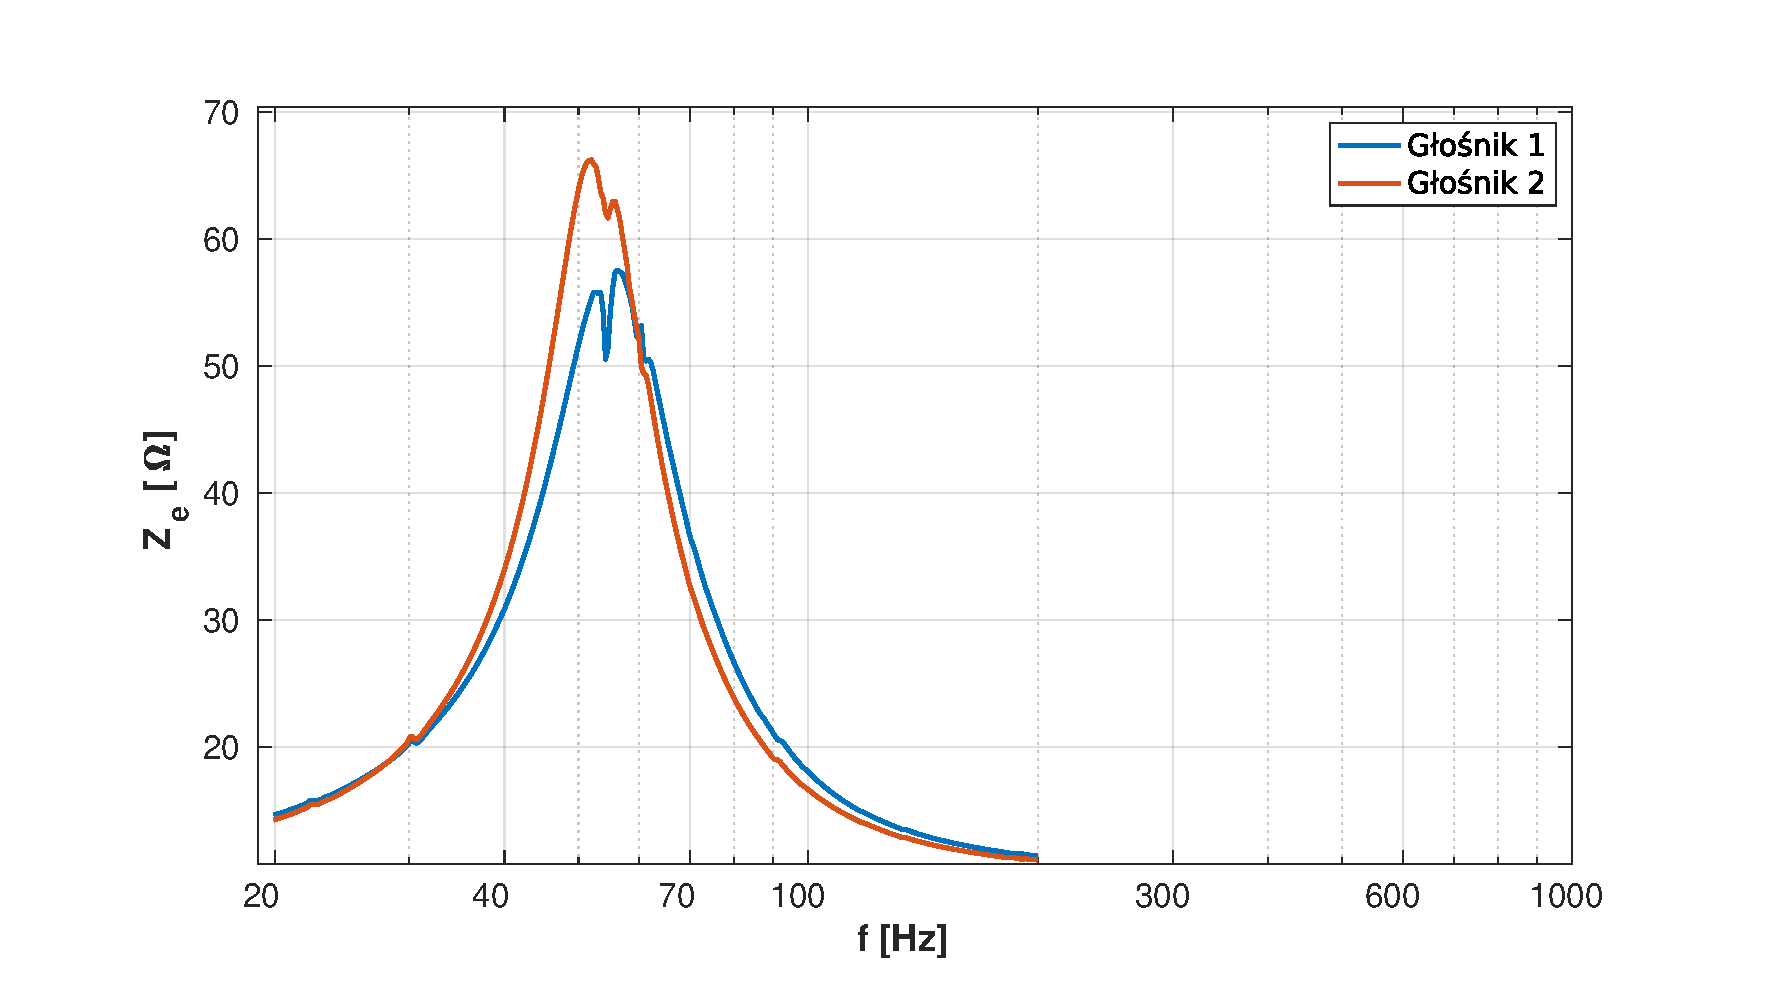
\includegraphics[width=.8\textwidth,trim={2cm .5cm 2cm 1cm},clip]{porownanie_glosnikow.pdf}
			\caption{Charakterystyki impedancji obu badanych głośników w~odgrodzie}
			\label{r:2glosniki}
		\end{figure}
		
		\begin{figure}[!ht]
			\centering
			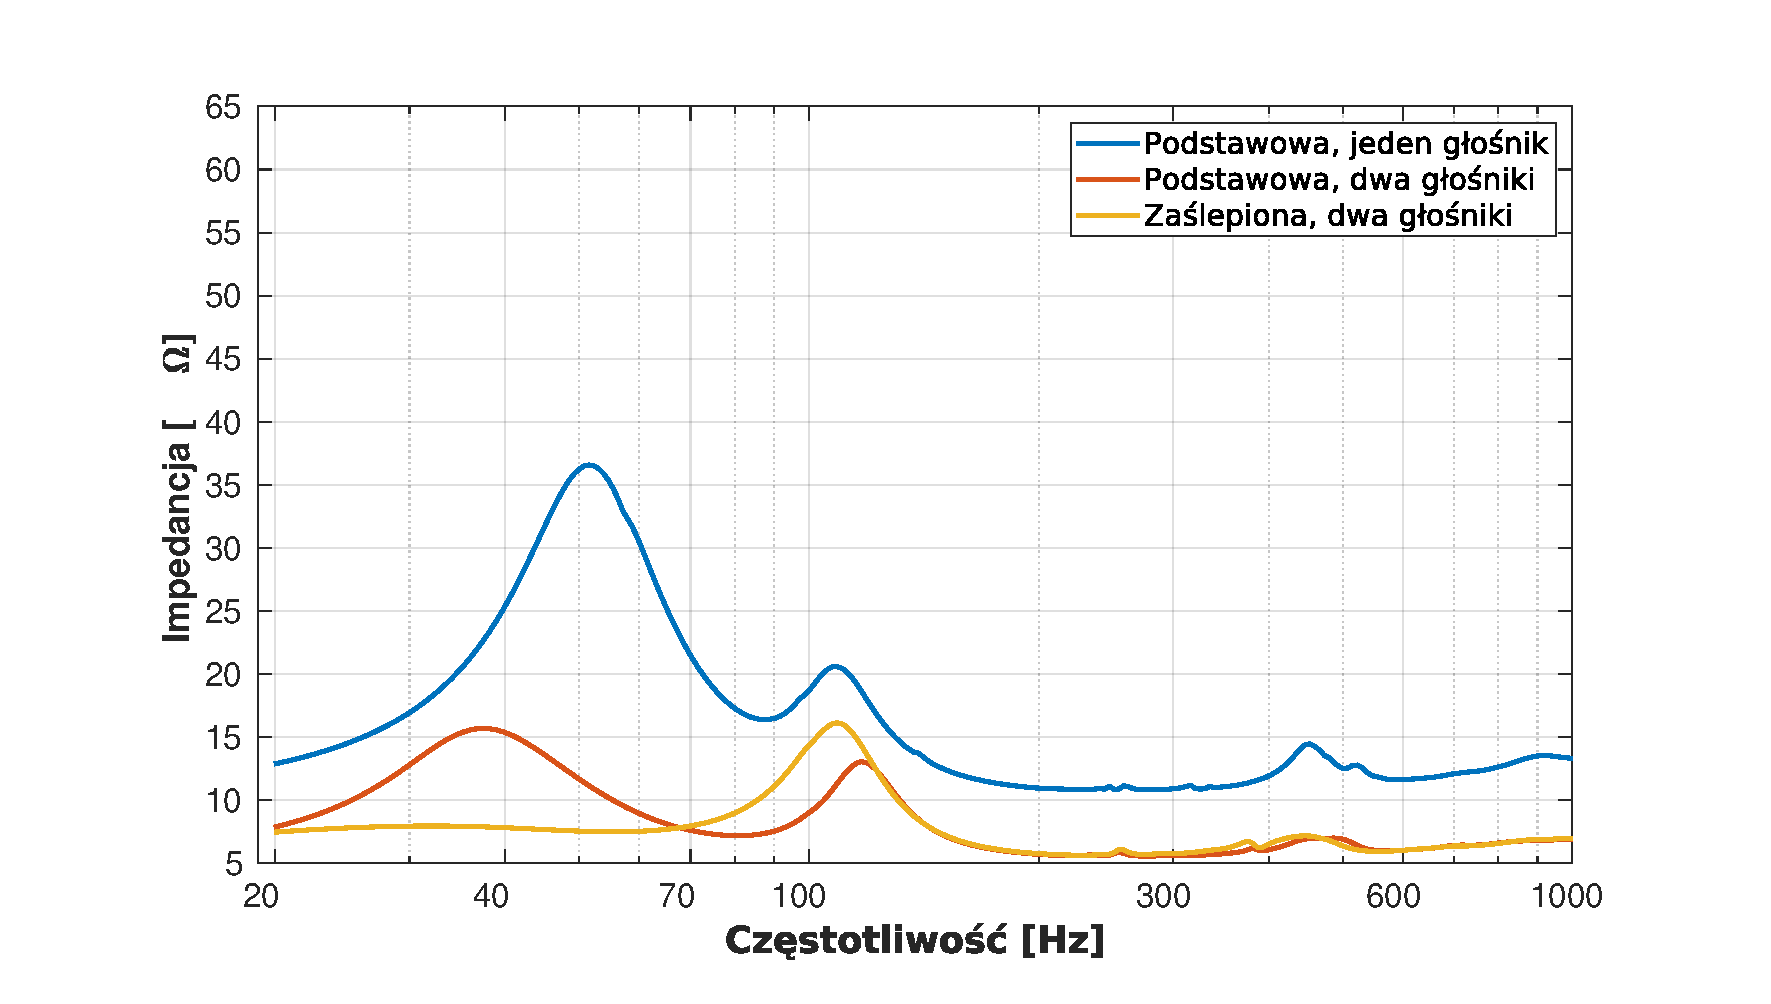
\includegraphics[width=.8\textwidth,trim={2cm .5cm 2cm 1cm},clip]{obudowa_otwory.pdf}
			\caption{}
			\label{r:obudowa_otwory}
		\end{figure}
		
	\subsection{Skuteczność}
		
		\begin{figure}[!ht]
			\centering
			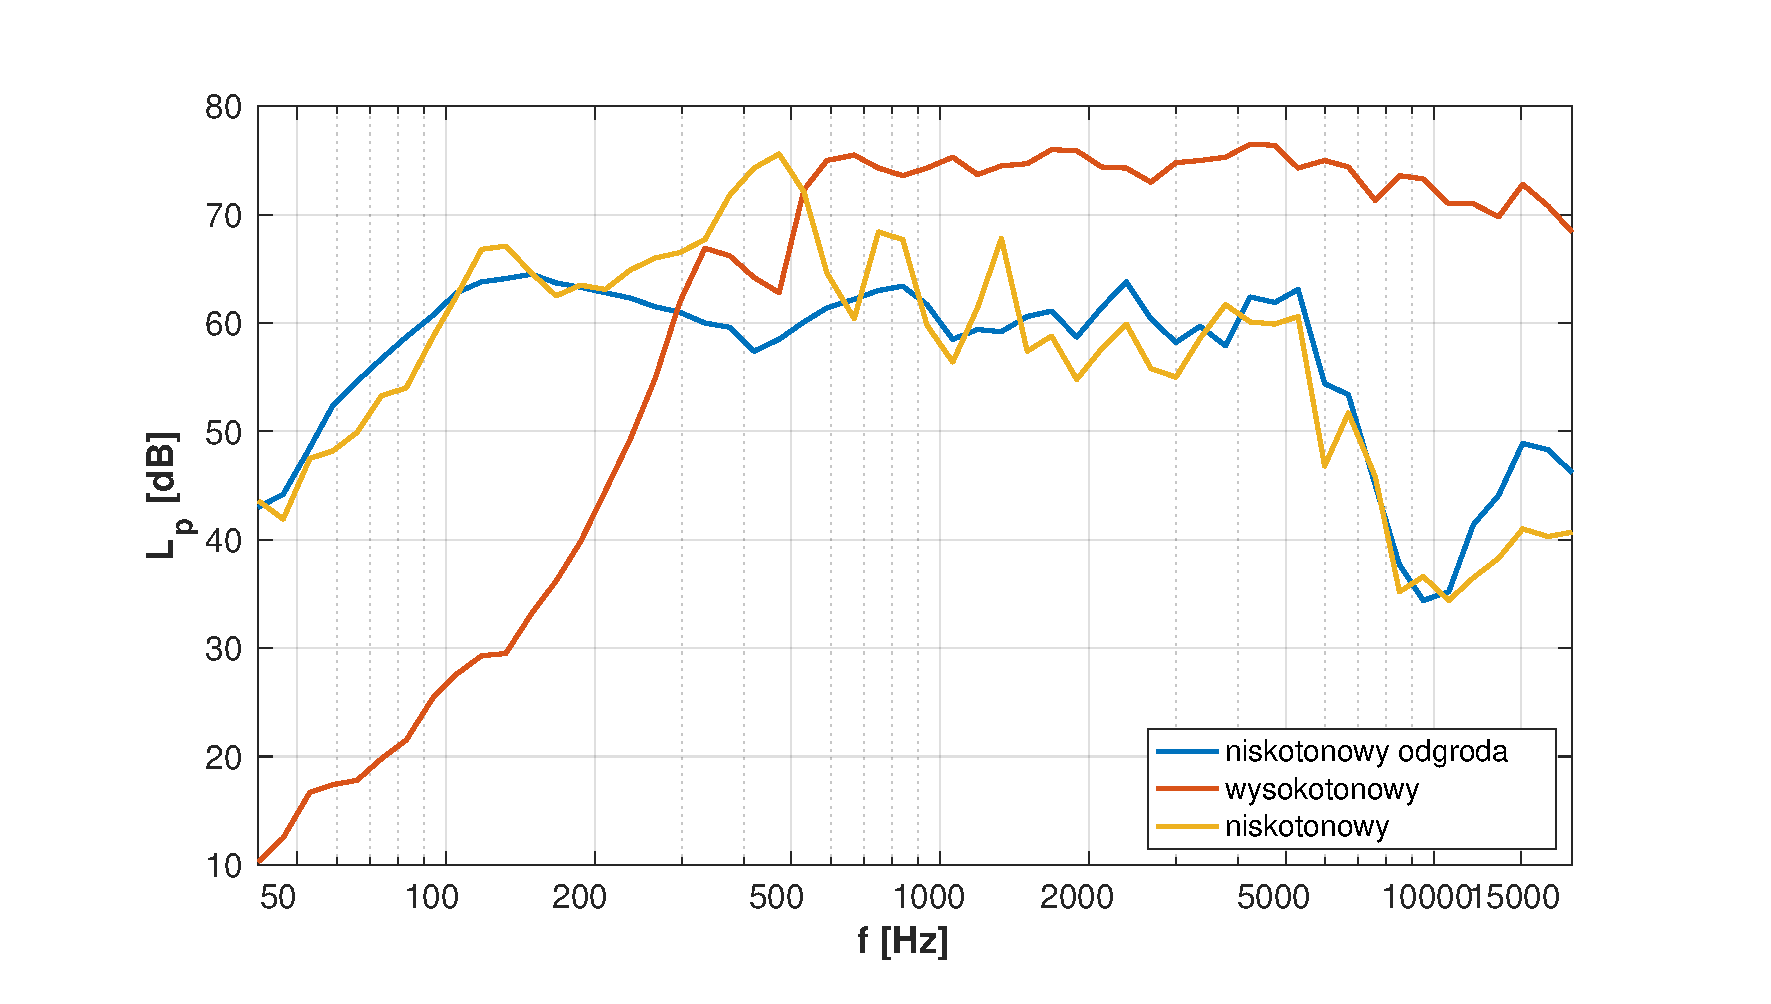
\includegraphics[width=.8\textwidth,trim={2cm .5cm 2cm 1cm},clip]{skutecznosci_stolik.pdf}
			\caption{}
			\label{r:skutecznosc}
		\end{figure}
		

		
		% + kierunkowość, skuteczność
	
	\subsection{Drgania obudowy}
		
		%generalnie nie widać zależności
		Analiza uzyskanych wyników nie dała podstaw do sformułowania zależności między obudową, a~charakterystykami amplitudowymi -- pomiędzy widmami sygnału z~wibrometru i~mikrofonów nie widać wyraźnych zależności. W~niektórych punktach pomiarowych można zauważyć zmiany kształtu charakterystyki dla tej samej częstotliwości, jednak są to raczej jednostkowe przypadki, na podstawie których nie można wysnuć ogólnych wniosków.
		
		Spośród zarejestrowanych przebiegów wybrano punkty \range{1}{4}, między którymi można dostrzec pewne zależności i~zestawiono je na rysunku~\ref{r:wibrometr_1-4}. W~punktach tych wyraźnie widoczny jest wzrost amplitudy przemieszczeń w~paśmie \SI{260}{\hertz}; jednocześnie w~tym samym paśmie zauważalny jest spadek poziomu ciśnienia akustycznego. Wybrane punkty zlokalizowane są na dwóch różnych ściankach obudowy, jak pokazano na rysunku~\ref{r:wibro_pkt} \comment{rozwinięcie myśli?}
		
		\begin{figure}[!ht]
			\centering
			\adjincludegraphics[width=.8\textwidth,trim={2cm .5cm 2cm 1cm},clip]{pkt1_4.pdf}
			\caption{Znormalizowane widma amplitudy przemieszczeń obudowy (góra) oraz poziomu ciśnienia akustycznego w~niewielkiej odległości od zestawu w~punktach pomiarowych~\range{1}{4}}
			\label{r:wibrometr_1-4}
		\end{figure}
		
		\begin{figure}[!ht]
			\centering
			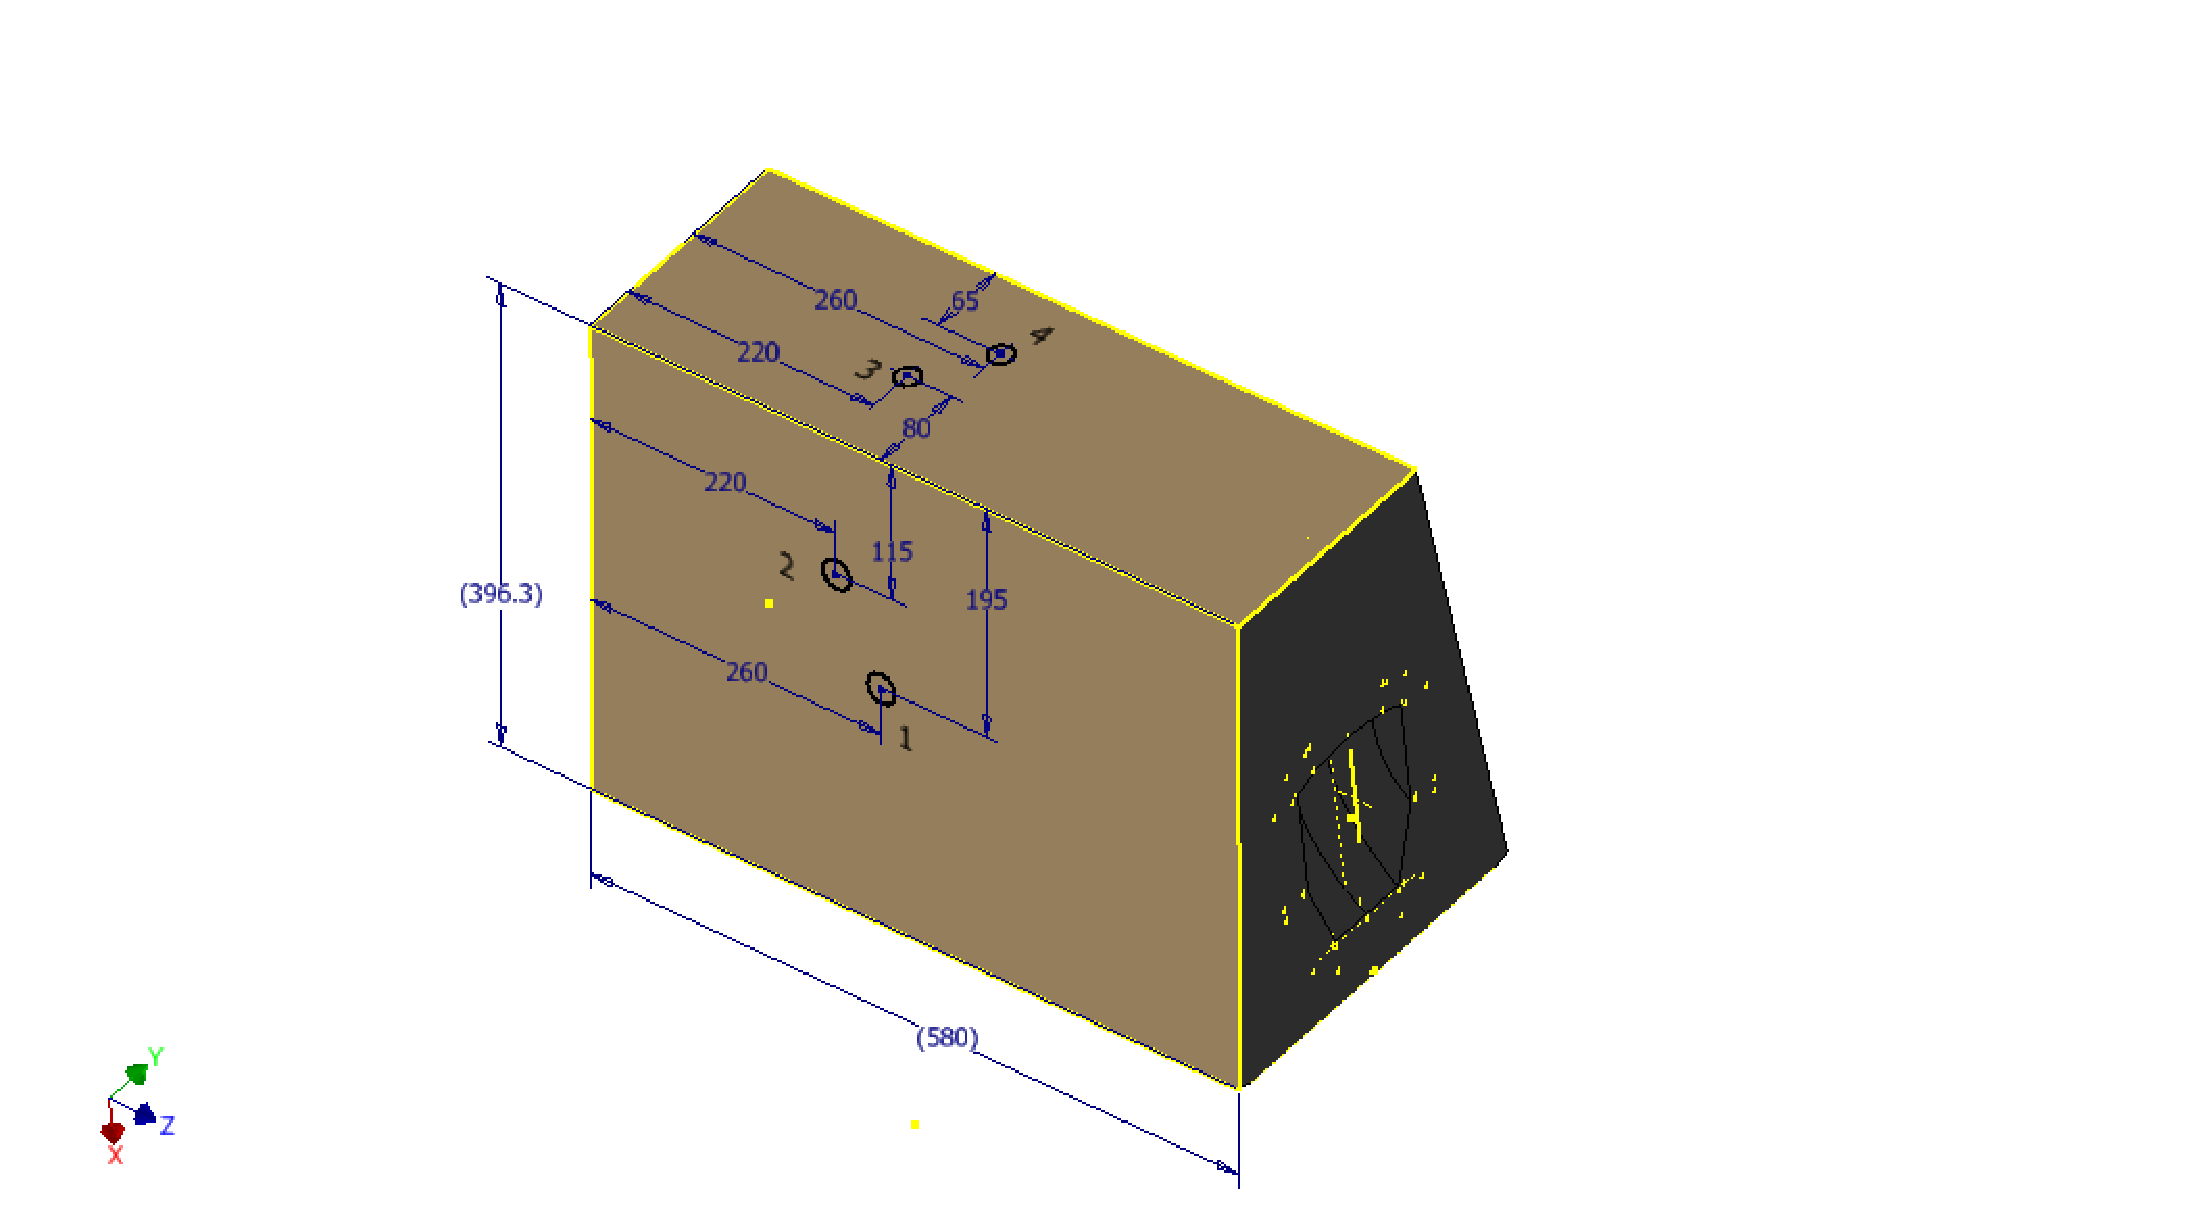
\includegraphics[width=.8\textwidth,trim={5cm .3cm 5cm 2.7cm},clip]{wibrometr.pdf}
			\caption{Rozmieszczenie punktów pomiarowych \range{1}{4} na obudowie (widok tylnej i~górnej ścianki)}
			\label{r:wibro_pkt}
		\end{figure}
		
		Kolejnym punktem, dla którego zdecydowano się zaprezentować wyniki jest punkt~\num{5}, zlokalizowany na uchwycie (na rysunku~\ref{r:wibro_pkt} po prawej stronie). Na widmie przemieszczeń (rys.~\ref{r:wibrometr_5}) widoczne jest lokalne maksimum amplitudy dla częstotliwości~\SI{400}{\hertz}, co jednak nie znajduje odzwierciedlenia w~widmie poziomu ciśnienia akustycznego -- mimo że podbicie tej częstotliwości jest widoczne w~charakterystykach skuteczności uzyskanych z~innych pomiarów~\ref{ss:w-skutecznosc}.%Drgania obudowy mogą mieć wpływ na pole akustyczne wokół zestawu.
		
		\begin{figure}[!ht]
		\centering
		\adjincludegraphics[width=.8\textwidth,trim={2cm .5cm 2cm 1cm},clip]{pkt5.pdf}
		\caption{Znormalizowane widma amplitudy przemieszczeń obudowy (góra) oraz poziomu ciśnienia akustycznego w~niewielkiej odległości od zestawu w~punkcie pomiarowym~\num{5}}
		\label{r:wibrometr_5}
		\end{figure}
		
		Otrzymane wyniki nie dają podstaw do jednoznacznego wskazania wpływu drgań obudowy na charakterystykę głośnika. Jednocześnie do dalszej analizy tej zależności wskazane jest wykonanie pomiarów w~większej liczbie punktów oraz obliczeń statystycznych.

\section{Podsumowanie}

\printbibliography

\end{document}
